\documentclass[a4paper,11pt]{report}
\usepackage[T1]{fontenc}
\usepackage[utf8]{inputenc}
\usepackage{lmodern}
\usepackage[francais]{babel}
\usepackage{graphicx}
\usepackage{array}

\title{}
\author{}

\begin{document}

\maketitle
\tableofcontents

\begin{abstract}
\end{abstract}

\chapter{Partie réseau}

\section{Modélisation des classes de réseau}

\subsection{UML de gestion des clients pour le serveur}

    \begin{figure}[th]
      \begin{center}
        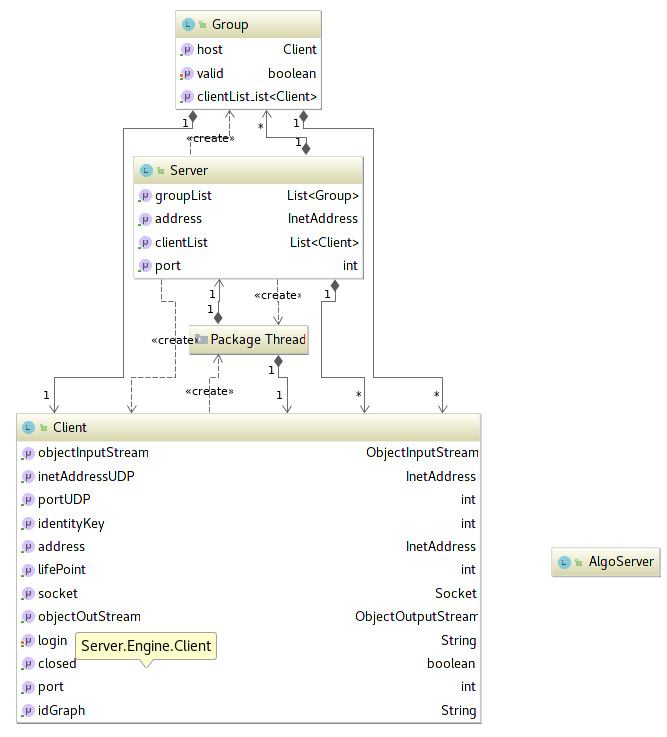
\includegraphics[scale=0.6]{Assets/UML_serveur.png}
        \caption{UML du serveur}
        \label{UML du serveur}
      \end{center}
    \end{figure}
    
    
    Comme illustré sur le diagramme ULM (\textit{figure~\ref{UML du serveur}}) le serveur contient des clients et des groupes et les groupes contiennent eux même des clients.
Un groupe possède en variable d’instance son hôte. 
Un client possède les flux objets, son socket et ses coordonnées pour le transport UDP.
Et le serveur son socket serveur TCP et UDP.





\subsection{UML de gestion des données pour les clients}
 \begin{figure}[th]
      \begin{center}
        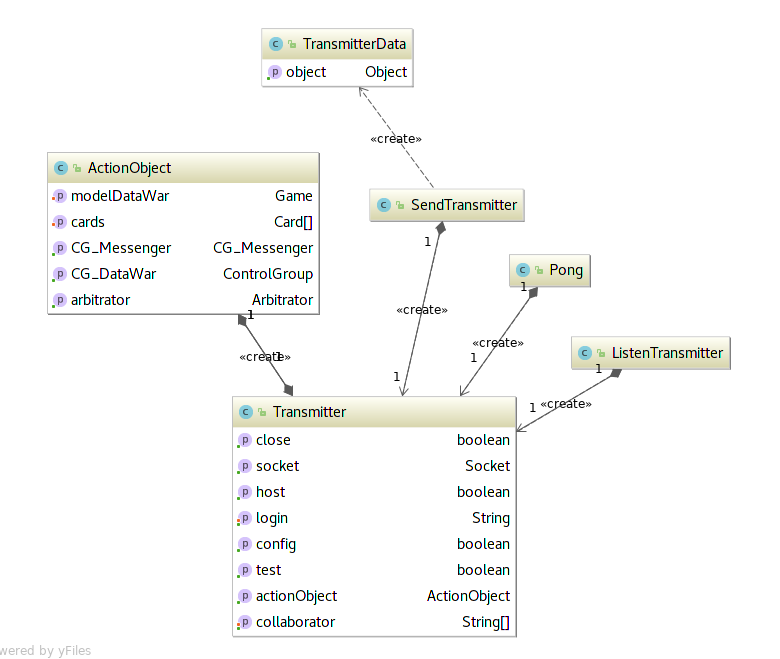
\includegraphics[scale=0.6]{Assets/UML_client.png}
        \caption{UML du client}
        \label{UML du client}
      \end{center}
    \end{figure}
    
  Comme illustré sur le diagramme ULM (\textit{figure~\ref{UML du client}}) le \textit{Transmitter} a pour variable d’instance son socket de connexion, ses flux objets, la liste des logins des membres du groupe. La variable host permet de savoir le mode hôte ou invité sur le groupe et la variable test sert aux tests logiciels. Un \textit{Transmitter} possède un \textit{ActionObject} et un \textit{ActionObject} possède un \textit{Transmitter}. La classe \textit{ActionObject} contient les contrôles groupes des applications qu’elle fait fonctionner en réseau : \textit{Messenger}, et le \textit{DataWar}.



\section{Les classes annexes}

\subsection{Visualisation de la situation du serveur}

    \begin{figure}[th]
      \begin{center}
        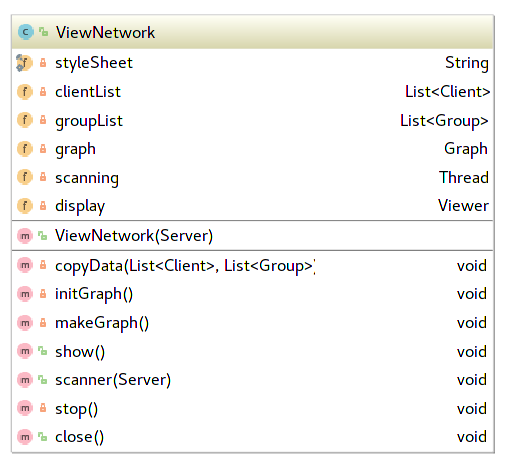
\includegraphics[scale=0.4]{Assets/UML_Network.png}
        \caption{Classe ViewNetwork}
        \label{Classe ViewNetwork}
      \end{center}
    \end{figure}
    
    La classe \textit{ViewNetwork} (Voir la \textit{figure~\ref{Classe ViewNetwork}}) permet une visualisation en temps réel de la situation du serveur. Elle montre dans une fenêtre un graphe avec pour nœud les clients et leur groupe pour liaisons. Le graphe est créé avec la librairie \textit{GraphSteam}. Lors de la création de la classe un thread est lancé pour réactualiser le graphe sur l’état du serveur. La fréquence réactualisation est de 500 millisecondes.

\subsection{Communication avec la base de donnée}

  \begin{figure}[th]
      \begin{center}
        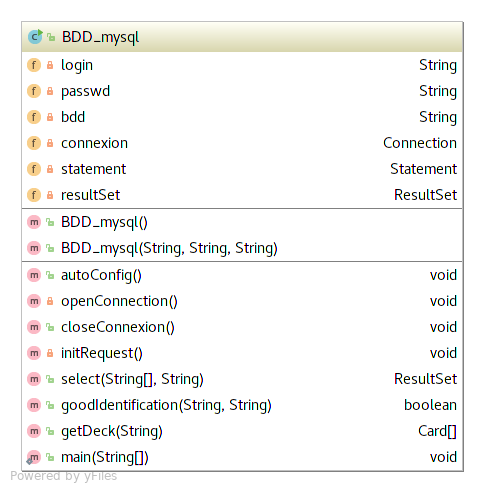
\includegraphics[scale=0.4]{Assets/UML_BDD.png}
        \caption{Classe BDD\_mysql}
        \label{Classe BDD_mysql}
      \end{center}
    \end{figure}
    
    La classe \textit{BDD\_mysql} (Voir la \textit{figure~\ref{Classe BDD_mysql}}) permet d’accéder simplement à la base de donnée du serveur. La classe utilise le package \textit{mysql\_connector} pour accéder à la base de donnée et exécuter les recettes SQL. La classe possède des fonctions permettant de savoir si un utilisateur est correctement identifié, ou encore la récupération du deck d’un joueur sous forme objet.




\section{Organisation et fonctionnement des communications}

\subsection{Organisation des communications}
Dans cette partie sera présenté le fonctionnement et l’organisation des communications du module de gestion du réseau.

\subsubsection{Organisation physique des communications}

L’organisation physique des communications est représenté sur le schéma en \textit{figure~\ref{schémaCom}} avec sa légende en \textit{figure~\ref{leSchémaCom}}
  
  \begin{figure}[th]
      \begin{center}
        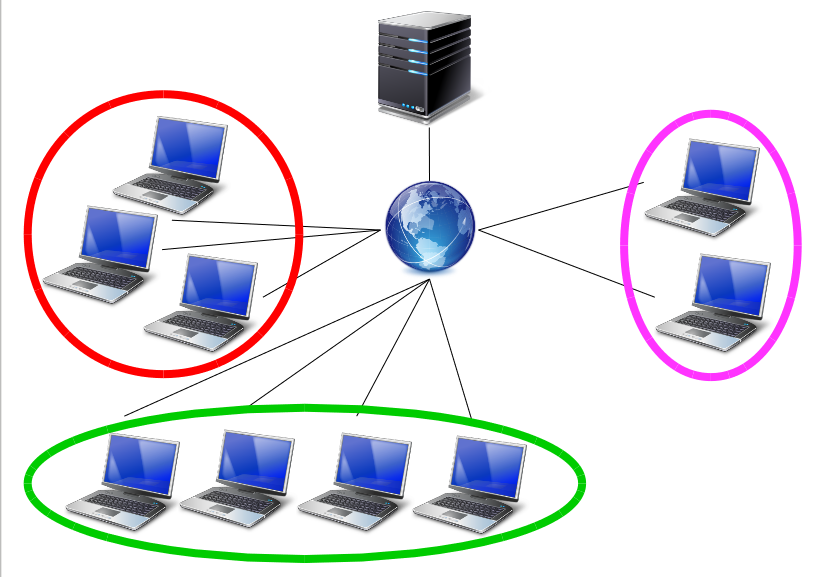
\includegraphics[scale=0.4]{Assets/s_r_1.png}
        \caption{Schéma montrant les communications physique}
        \label{schémaCom}
      \end{center}
    \end{figure}

   \begin{figure}[th]
      \begin{center}
        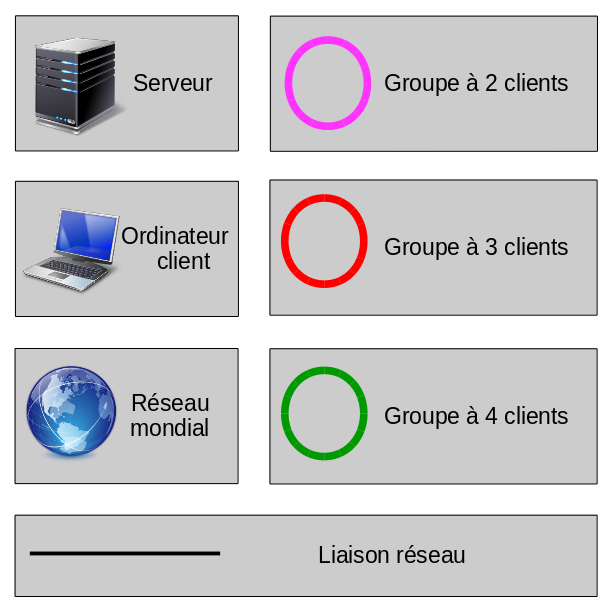
\includegraphics[scale=0.4]{Assets/l_r_1.png}
        \caption{Légende du schéma montrant les communications physique}
        \label{leSchémaCom}
      \end{center}
    \end{figure}
    
  
  Une fois que les groupes sont configurés est créé le serveur établi les communications entre les différents membres d’un groupe, il a le rôle de relai. Ce fonctionnement par relai permet de communiquer dans des zones avec des par-feus très restrictifs.
Le serveur est capable de gérer plusieurs groupes en même temps et de différente taille entre 2 et 4 membres. Mais deux clients appartenant chacun à un groupe différant ne peuvent pas communiquer entre eux.

\subsubsection{Organisation logicielle des communications}

  Un client communique simultanément avec tous les autres clients, ils ne peuvent pas parler un à un. Ceci pour facilité simplement la synchronisation des données du modèle du jeu, et la gestion des avaries lors de déconnexion éventuel. De cette façon le client n’a pas besoin de savoir qui est encore connecté pour envoyer les données. (la synchronisation et les avarie seront expliqué plus tard).
  
\subsection{Fonctionnement des communications}

\subsubsection{Classes de communication}
Le tableau \ref{tab1comClasses} récapitule les classes pour transmettre des objets :

  \begin{table}
    \begin{center}
      \begin{tabular}{|c|c|c|}
         \hline \textbf{Action}&\textbf{Classe du serveur}&\textbf{Classe du client} \\
         \hline Attendre de recevoir&\textit{ListenClient\_Wait}&- \\
         \hline Attendre d’envoyer&\textit{SendClient\_Wait}&- \\
         \hline Recevoir&\textit{ListenClient}&\textit{ListenTransmitter} \\
         \hline Envoyer&\textit{SendClient}&\textit{SendTransmitter}\\
         \hline
      \end{tabular}
      \caption{Tableau récapitulant les classes pour les transmissions objet}  
      \label{tab1comClasses}
    \end{center}
  \end{table}
  
  Les classes pour attendre de recevoir ou d’envoyer des données sont les classes mères des classes pour envoyer ou recevoir des données. La différence avec les classes filles est qu’elle implémente \textit{Runnable} pour pouvoir être threader.

\subsubsection{Procédure de communication communication entre membre d’un groupe}
Cette procédure permet à un client de communiquer avec les autres membres de son groupe.
\begin{description}
  \item[1) Envoie des données du client vers le serveur]
    \textit{\\Classe : Transmitter - Fonction : speakTransmitters()\\}
	  Pour envoyer un objet quelconque il suffit d’appeler cette méthode et de passer en paramètre l’objet à envoyer à destination du serveur pour une retransmission. Cette méthode est synchronized pour être certain que l’on ne puisse pas envoyer des données dans le désordre au avoir des conflits avec d’autre méthode de communication. Les données à envoyer sont encapsulés dans une classe TransmitterData.
	
	\item[2) Réception des données des clients]
	\textit{\\Classe : ListenClient - Fonction : run()\\}
	  Le serveur attend des objets sur le flux objet de chaque client, soit un thread d ‘écoute par client.
Dans cette méthode lorsqu’un objet est reçu, le serveur vérifie le type de données avant de la retransmettre. Si un nombre trop important d’erreur venait à se produire, la méthode fermerait le socket du client en question.

  \item[3) Retransmission des données du serveur vers les clients]
  \textit{\\Classe : Group - Fonction : clientSpeakGroup()\\}
    Une fois la réception d’un objet  \textit{TransmitterData} le serveur retransmet les données aux autres membres du groupe. Cette méthode est elle aussi  \textit{synchronized} pour les mêmes raisons que la méthode possédante. Pour réaliser son traitement la méthode à besoin de l’objet à transmettre et le client émetteur pour ne pas lui retourner les données.
    
  \item[4) Réception des données du serveur]
  \textit{\\Classe : ListenTransmitter - Fonction : run()\\}
    Le client attend des objets dans cette fonction. Si un objets est reçu il est envoyé dans la classe \textit{Transmitter} par la méthode \textit{readObject()} pour être traité. Si des erreurs sont constatés le socket est fermé.
\end{description}

\subsubsection{Procédure de communication direct avec le serveur}
  Cette procédure permet à un client de réaliser des actions enregistrées dans le serveur par le développer.

\begin{description}
  \item[1) Classe : Transmitter - Fonction : speakServer()]
    \textit{\\Classe : Transmitter - Fonction : speakTransmitters()\\}
	  Cette méthode à pour bute de transmettre au serveur le signal (un Integer) au serveur. Pour cela la méthode encapsule le signal dans l’objet ServerMessage. L’objet est transmit par les flux objets du Transmitter dans un thread.
	
	\item[2) Réception du signal par le serveur]
	\textit{\\Classe : ListenClient - Fonction : run()\\}
	  La réception du signal ce fait ici au même endroit que la réception des données de groupe. Si l’objet reçu est une instance de  ServerMessage, alors il est transmit a la classe serveur pour être traité.

  \item[3) Traitement du signal]
  \textit{\\Classe : processingMessage - Fonction : run()\\}
  Cette méthode exécute l’instruction correspondante au numéro de signal dans l’objet ServerMessage.
\\Pour le moment deux signaux sont répertoriés dans le tableau \ref{tab2signal}:

\newcolumntype{M}[1]{>{\raggedright}m{#1}}
\begin{table}

    \begin{center}
      \begin{tabular}{|l|M{12cm}|}
         \hline \textbf{Signal}&\textbf{Action}\tabularnewline
         \hline 6&Ordonne la fermeture du signal si le code contenue dans la classe est correcte.\tabularnewline
         \hline 5&Recherche les cartes du groupe dans la base de donnée avec la classe \textit{BDD\_mysql} et la méthode \textit{getDeck()}. Puis les cartes sont retournées par flux d’objet à l’émetteur du signal.\tabularnewline
         \hline
      \end{tabular}
      \caption{Tableau récapitulant les type de signaux du serveur}  
      \label{tab2signal}
    \end{center}
  \end{table}
    
\end{description}

  
\subsection{Protocole de création d’un groupe}

  Sur l'organigramme en figure \ref{organiGroupe} est présenté la procédure de création d’un groupe de jeu sur le serveur.

  \begin{figure}[th]
      \begin{center}
        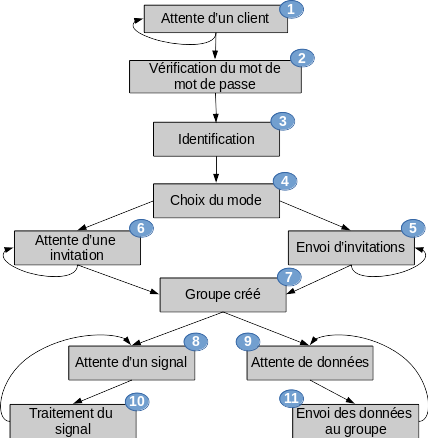
\includegraphics[scale=0.9]{Assets/creationGroup.png}
        \caption{Organigramme montrant les étapes de la création d'un groupe}
        \label{organiGroupe}
      \end{center}
    \end{figure}

\newcolumntype{M}[1]{>{\raggedright}m{#1}}
  
  \begin{table}
    \begin{center}
      \begin{tabular}{|l|M{9cm}|M{2.5cm}|}
      
       \hline \textbf{Numéro}&\textbf{Action}&\textbf{Classes utilisées}\tabularnewline
         
        \hline 
        1&Cette étape consiste à attendre un client, créer un socket, puis ouvrir un flux objet provisoire entrant. Si le port et l’adresse sont enregistrés dans la liste forcing alors le client est déconnecté.&\textit{WaitClients}\\\textit{Server}
        \tabularnewline

        
        \hline 
        2&Le serveur attend la clef d’accès envoyer par le client.
Si la clef est incorrecte le client est déconnecté, puis son adresse et son port sont stockés dans la liste forcing pour que la personne ne puisse pas forcer la clef. Sinon les flux objet entrant et sortant sont créés ainsi que les classes \textit{Ping} et \textit{Pong}.&\textit{Server}\\\textit{Ping}/\textit{Pong}\\\textit{Client}\\\textit{BDD\_mysql}
        \tabularnewline
        
        \hline
        3&L’étape d’identification consiste à recevoir le login et le mot de passe du client.\\
        -Si elle ne correspond pas à la base de donnée o  si la même personne est déjà connecté le socket est fermé.\\
        -Si l’identification est correcte un message de sucés est envoyé.&\textit{Server}\\\textit{Client}\\\textit{InfoProtocol}
        \tabularnewline
        
        \hline
        4&Cette étape consiste à demander au client quelle mode de création de groupe souhaite-t-il.\\
Si le client revoie yes, alors un groupe est créé ou il en est hôte. Sinon le client est mis en attente d’acceptation d’un groupe.&\textit{Server}\\\textit{Group}\\\textit{InfoProtocol}
        \tabularnewline
        
        
        \hline
        5&Une liste de tout les clients en attente d’invitation est envoyé a l’hôte. L’hôte peut envoyer une invitation à un client en attente d’invitation en envoyant le nom de la personne concerné au serveur, puis le serveur transmet l’invitation. L’hôte peut envoyer le message de fin de configuration et si la taille du groupe est entre 2 et 4 personnes le groupe est validé.&\textit{Server}\\\textit{Client}\\\textit{InfoProtocol}
        \tabularnewline
        
        \hline
        6&Le serveur transmet toutes les invitations au client avec un délai de 12 secondes maximum pour répondre.\\ 
Si le client renvoi l’invitation il est placé dans le groupe de l’émetteur et attend la validation du groupe.\\
Si il la refuse il ne renvoie rien.\\
Si le temps est dépassé le serveur n’acceptera pas une éventuelle acceptation cette invitation.&\textit{Server}\\\textit{Group}\\\textit{Client}\\\textit{Transmitter}\\\textit{InfoProtocol}
      
        \tabularnewline
        
        \hline
        7&Lorsque l’hôte valide le groupe un message de confirmation de sa création est envoyé à tous ses membres. Ainsi qu’une liste du nom de tout ses membres.&\textit{Server}\\\textit{Group}\\\textit{InfoProtocol}
        \tabularnewline
        
        \hline
        8&Le serveur attend un signal contenu dans l’objet \textit{ServerMessage} émis par un des membres du groupe.&\textit{ServerMessage}\\\textit{Server}
        \tabularnewline
        
        \hline
        9&Le serveur attend des donnés contenus dans l’objet \textit{TransmitterData}.&\textit{TransmitterData} \\\textit{Server}
        \tabularnewline
        
        \hline
        10&Suivant ce signal le serveur exécute une procédure bien précise.\\\textit{Exemple : le signal 5 correspond a l’envoi des cartes du jeu.}\\&\textit{Server}\\\textit{Client}
        \tabularnewline
        
        \hline
        11&Le serveur retransmet les données aux membres du groupe.&\textit{Group}
        \tabularnewline
        
        \hline
      
      \end{tabular}
      \caption{Tableau expliquant les étapes de l'organigramme \textit{(figure~\ref{organiGroupe})}}  
      \label{tabOrganigramme}
    \end{center}
  \end{table}


\end{document}
